\section{}

\textbf{Tiempo de lectura:} \{s19-reading-time\}

Como hemos comentado, cada volumen puede albergar un sistema de
archivos. A continuación estudiaremos los elementos más comunes a la
mayor parte de los sistemas de archivos actuales.

\section{Estructura de un sistema de
archivos}\label{_estructura_de_un_sistema_de_archivos}

\begin{figure}
\centering
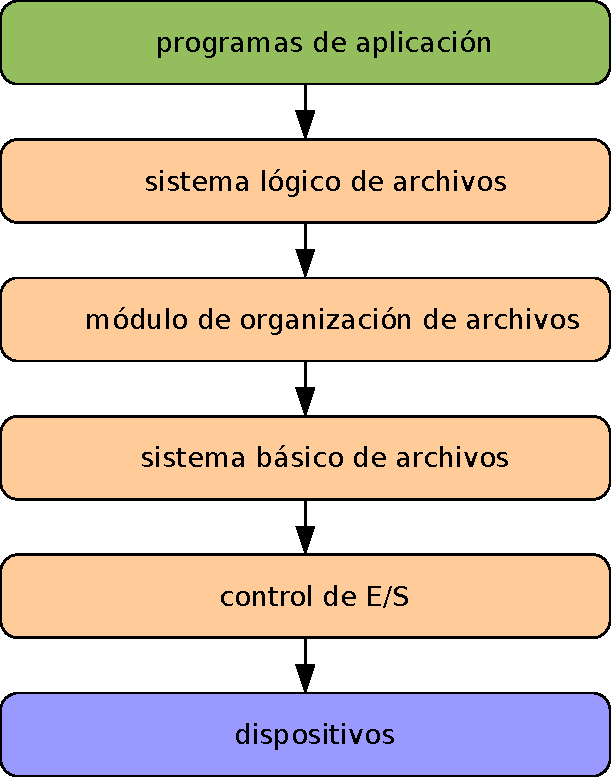
\includegraphics[width=0.8\textwidth]{media/C19_sistema_de_archivos/estructura_sistema_de_archivos.pdf}
\caption{Estructura de un sistema de
archivos.}\label{fig-estructura-sistema-de-archivos}
\end{figure}

Los sistemas de archivos son un componente complejo, por lo que suelen
estar compuesto de varios niveles diferentes. En la
\hyperref[fig-estructura-sistema-de-archivos]{Estructura de un sistema
de archivos.} se muestra un ejemplo típico de la estructura de un
sistema de archivos diseñado en niveles. Cada nivel utiliza las
funciones de los niveles inferiores y proporciona nuevas funciones a los
niveles superiores.

\subsection{Control de E/S}\label{_control_de_es}

{} En el nivel más bajo, accediendo directamente a los dispositivos de
almacenamiento, se encuentra el \textbf{control de E/S}.

Contiene los controladores de dispositivo encargados de transferir la
información entre la memoria principal y el disco. Estos controladores,
que generalmente son compartidos entre los distintos sistemas de
archivos, transfieren los datos en unidades de \textbf{bloques}{} ---en
lugar de transferir un byte cada vez--- para mejorar la eficiencia. Cada
\_*bloque* está formado por uno o más sectores.

Dependiendo de la unidad de disco, los sectores pueden tener tamaños de
entre 32 bytes y 4096 bytes. Lo más común es que su tamaño sea de 512
bytes.

\subsection{Sistema básico de
archivos}\label{_sistema_buxe1sico_de_archivos}

{} El \textbf{sistema básico de archivos} se encarga de enviar comandos
genéricos al controlador de dispositivo apropiado, con el fin de leer y
escribir bloques físicos en el disco. Cada bloque físico se identifica
mediante su dirección de disco numérica.

Por ejemplo, en dispositivos que usan direccionamiento de tipo
cabeza-cilindro-sector (CHS), la dirección de un sector podría ser:
unidad 1, cilindro 73, cabeza 2, sector 10. Mientras que en dispositivos
que admiten direccionamiento LBA (\emph{Logical Block Addressing}), la
dirección de un sector podría ser: unidad 1, sector 4691123.

El \textbf{{}LBA} es un método común para especificar la localización de
los sectores de un disco. Usa un esquema de direccionamiento lineal,
donde cada sector es identificado con un número entero único. Antes de
este método, se usaba el de cabeza-cilindro-sector (CHS), pero tenía la
desventaja de hacer públicos los detalles físicos del dispositivo de
almacenamiento.

\subsection{Módulo de organización de
archivos}\label{_muxf3dulo_de_organizaciuxf3n_de_archivos}

{} El \textbf{módulo de organización de archivos} tiene conocimiento de
los archivos y se encarga de traducir las direcciones lógicas de los
bloques en los archivos ---es decir, posición del bloque dentro del
archivo, siendo 0 la dirección del primer bloque--- en las direcciones
físicas de bloque ---por ejemplo, cilindro, cabeza y sector del bloque
correspondiente en el dispositivo de almacenamiento--- que serán
enviadas al \textbf{sistema básico de archivos} para que realice las
transferencias solicitadas.

Los bloques lógicos de cada archivo son numerados de 0 a \emph{N}, pero
los bloques físicos asignados a estos bloques lógicos no tienen por qué
coincidir en los números de bloque. Por eso, el \textbf{módulo de
organización de archivos} debe utilizar la ubicación del contenido del
archivo en el disco y la información sobre los bloques físicos
asignados, para traducir las direcciones lógicas en direcciones físicas.

Además, el módulo de organización, incluye el gestor de espacio libre,
que controla los bloques no asignados y proporciona dichos bloques
cuando el \textbf{módulo de organización de archivos} lo necesita, ya
sea para crear un archivo nuevo o para extender uno existente.

\subsection{Sistema lógico de
archivos}\label{_sistema_luxf3gico_de_archivos}

El \textbf{sistema lógico de archivos} gestiona los \textbf{metadatos}.
En los \textbf{{}metadatos} se incluye toda la estructura del sistema de
archivos, excepto los propios datos de los archivos.

Entre dichos \textbf{metadatos} está la \textbf{estructura de
directorios} y los \textbf{bloques de control de archivo}. Un
\textbf{bloque de control de archivo}{} o \textbf{{}FCB} (\emph{File
Control Block}) contiene información acerca del archivo, incluyendo su
propietario, los permisos y la ubicación del contenido del mismo.

Además, el \textbf{sistema lógico de archivos} también es responsable de
las tareas de protección y seguridad.

Cada sistema operativo puede soportar uno o más sistemas de archivos
para dispositivos de disco. Por ejemplo, en los sistemas UNIX se utiliza
el «sistema de archivos UNIX» o \{ufs\} (\emph{UNIX File System}), que
está basado en el sistema \{ffs\} (\emph{Fast File System}) de la
Universidad de Berkeley. Microsoft Windows soporta los sistemas de
archivo \{fat\} (\emph{File Allocation Table}), \{fat32\} y \{ntfs\}
(\emph{NT File System}). En Linux se soportan más de cuarenta sistemas
de archivo, entre los que cabe destacar: la familia \emph{extended
filesystem} --- \{ext2\}, \{ext3\} y \{ext4\}--- \{xfs\} y \{btrfs\}.

Además, la mayoría de los sistemas operativos modernos soportan otros
sistemas de archivo, como los utilizados en los soportes removibles. Por
ejemplo el \{iso9660\}, utilizado por la mayor parte de los CD-ROM, o el
\{udf\} (\emph{Universal Disk Format}), utilizado por los DVD-ROM y
Blu-ray.

\section{Estructuras de metadatos en
disco}\label{_estructuras_de_metadatos_en_disco}

Para implementar un sistema de archivos se utilizan diversas estructuras
de \textbf{metadatos} alojadas tanto en el disco como en la memoria.
Estas estructuras varían dependiendo del sistema operativo y del sistema
de archivos. Sin embargo, a continuación intentaremos describir
brevemente las estructuras en disco más comunes.

\subsection{Bloque de control de
arranque}\label{_bloque_de_control_de_arranque}

{} {} {} En todo sistema de archivos suele haber un \textbf{bloque de
control de arranque} ---también llamado \textbf{bloque de inicio} o
\textbf{sector de arranque}--- que suele ocupar el primer bloque de cada
volumen y que contiene la información necesaria para iniciar un sistema
operativo a partir de dicho volumen.

Este bloque puede estar vacío, si el volumen no contiene un sistema
operativo.

\subsection{Bloque de control de
volumen}\label{_bloque_de_control_de_volumen}

{} El \textbf{bloque de control de volumen} contiene todos los detalles
acerca del volumen. Por ejemplo, el número máximo de bloques, el tamaño
de los bloques, el número de bloques libres y punteros a los mismos; así
como un contador de bloques de información \textbf{FCB} ocupados y
punteros a estos.

A esta estructura se la denomina \textbf{{}superbloque}, en los sistemas
de archivos de sistemas UNIX y Linux. Mientras que en \{ntfs\} esta
información se almacena en la \textbf{tabla maestra de archivos} o
\textbf{{}MFT} (\emph{Master File Table}).

\subsection{Bloque de control de
archivo}\label{_bloque_de_control_de_archivo}

{} Todo sistema de archivos tiene un \textbf{bloque de control de
archivo} o \textbf{{}FCB} (\emph{File Control Block}) por archivo, en
que se almacenan numerosos detalles sobre cada uno de los archivos Por
ejemplo, los permisos, el propietario, el tamaño y la ubicación de los
bloques de datos, entre otros.

En términos generales, todos los \textbf{FCB} del sistema de archivos se
almacenan en una tabla denominada \textbf{directorio de dispositivo}{} o
\textbf{tabla de contenidos del volumen}{}.

En los sistemas de archivos de sistemas UNIX y Linux cada FCB se
denomina \textbf{{}inodo} y se almacenan a continuación del
\textbf{superbloque}. En \{ntfs\} esta información se almacena en la
\textbf{MFT}, ya que cada entrada de dicha tabla es un \textbf{FCB}.

\subsection{Estructura de directorios}\label{_estructura_de_directorios}

Finalmente, por lo general los sistemas de archivos tienen una
estructura de directorios, para organizar los archivos.

En los sistemas de archivos de sistemas UNIX y Linux, cada directorio es
como un archivo especial que almacena los nombres de los archivos que
contiene y los índices de los \textbf{inodos} de cada uno de ellos. En
\{ntfs\} es similar, aunque la estructura de directorios completa se
almacena en la propia \textbf{MFT}.

\section{Estructuras de metadatos en
memoria}\label{_estructuras_de_metadatos_en_memoria}

La información almacenada en memoria se utiliza tanto para la gestión
del sistema de archivos como para mejorar el rendimiento del mismo
mediante mecanismos de caché.

Los datos se cargan en el momento de comenzar a utilizar el sistema de
archivos ---proceso denominado montaje--- y se descartan cuando se va a
dejar de hacer uso del mismo ---es decir, en el desmontaje---.

Las estructuras existentes en la memoria pueden incluir las que a
continuación se describen:

\begin{itemize}
\item
  Una \textbf{tabla de montaje}{} en memoria que contiene información
  acerca de cada volumen montado en el sistema.
\item
  Una caché en memoria de la \textbf{estructura de directorios} que
  almacena la información relativa a los directorios a los que se ha
  accedido recientemente. Los directorios que actúan como puntos de
  montaje pueden contener un puntero a la entrada, en la tabla de
  montaje, del volumen montado en el directorio.
\item
  La \textbf{tabla global de archivos abiertos}{} que contiene una copia
  del \textbf{FCB} de cada archivo abierto en el sistema, además de
  otras informaciones.
\item
  La \textbf{tabla de archivos abiertos}{} de cada proceso. El
  \textbf{PCB} de cada proceso contiene una tabla donde se listan los
  archivos abiertos por el proceso.
\end{itemize}

La \textbf{tabla de archivos abiertos} contiene, para cada archivo, un
puntero a la entrada correspondiente del mismo archivo en la tabla
global de archivos abiertos, pero también guarda otras informaciones
adicionales que son particulares de cada proceso. Por ejemplo, si el
proceso lo ha abierto para lectura o escritura o la posición del puntero
que indica la siguiente posición a leer o escribir.

\section{Montaje de sistemas de
archivos}\label{_montaje_de_sistemas_de_archivos}

{} Un sistema de archivos debe \textbf{montarse} para que sus archivos
sean accesibles a los procesos del sistema. El proceso de montaje
incluye los siguientes pasos:

\begin{enumerate}
\def\labelenumi{\arabic{enumi}.}
\item
  Al sistema operativo se le debe proporcionar el nombre o identificador
  del dispositivo y el punto de montaje. El \textbf{punto de montaje}{}
  es la ubicación dentro de la estructura de directorios ---la ruta al
  directorio concreto--- a la que queremos conectar el sistema de
  archivos. Después de que el proceso de montaje se haya completado, los
  archivos y directorios del sistema de archivos montado serán
  accesibles como descendientes del directorio del \textbf{punto de
  montaje}.
\item
  A continuación el sistema operativo verifica que el dispositivo
  contiene un sistema de archivos válido. Para ello lee el
  \textbf{bloque de control de volumen} y comprueba que tiene un formato
  válido.
\item
  Finalmente el sistema operativo registra en la \textbf{tabla de
  montaje} el tipo de sistema de archivos y el identificador del
  dispositivo montado. Después, almacena el índice de la entrada
  correspondiente en la \textbf{tabla de montaje} en la copia en memoria
  del \textbf{FCB} del directorio que hace de \textbf{punto de montaje}.

  Esto permite que pueda ser recorrida la estructura de directorios de
  distintos sistemas de archivos, pasando de uno a otro de forma
  transparente, según sea necesario.
\end{enumerate}

En muchos sistemas operativos modernos, el montaje se ejecuta
automáticamente cuando los dispositivos son detectados durante el
arranque del sistema o cuando se conectan durante el funcionamiento del
mismo ---por ejemplo, cuando se inserta un medio en la unidad CD-ROM o
se pincha una memoria flash en un puerto USB---. En algunos se permite,
además, que el administrador del equipo ejecute operaciones de montaje
manuales.

\section{Archivos}\label{_archivos}

Cada sistema de archivos almacena en disco una tabla donde cada entrada
guarda un \textbf{bloque de control de archivo} o \textbf{FCB}
(\emph{File Control Block}) por archivo. Concretamente, en cada
\textbf{FCB} se almacena diversa información acerca del archivo al que
representa.

\subsection{Atributos de archivos}\label{_atributos_de_archivos}

La colección de atributos asociada a un archivo varía de un sistema
operativo a otro, pero típicamente son los siguientes:

\begin{itemize}
\item
  \textbf{Nombre}. Nombre simbólico del archivo, que se mantiene en un
  formato legible por la conveniencia de los usuarios.
\item
  \textbf{Identificador}. Identifica de forma unívoca el archivo dentro
  del sistema de archivos. Generalmente es el índice del \textbf{FCB} en
  la \textbf{tabla de contenidos del volumen}, donde se almacenan los
  \textbf{FCB}.
\item
  \textbf{Tipo}. Es un atributo necesario en los sistemas que soportan
  diferentes tipos de archivos.
\item
  \textbf{Ubicación}. Es un puntero a un dispositivo y a la ubicación de
  los bloques con los datos del archivo dentro del mismo.
\item
  \textbf{Tamaño}. Indica el tamaño actual de archivo ---en bytes,
  palabras o bloques--- y, posiblemente, el tamaño máximo permitido.
\item
  \textbf{Protección}. Información de control de acceso que determina
  quién puede leerlo, escribirlo, ejecutarlo, etc.
\item
  \textbf{Fecha, hora e identificación del usuario}. Esta información
  puede mantenerse para los sucesos de creación, de última modificación
  y último uso del archivo. Puede resultar útil para la protección,
  seguridad y monitorización del uso del archivo.
\end{itemize}

Los atributos de los archivos se almacenan en las estructuras de
\textbf{metadatos}.

Normalmente el nombre se almacena en la estructura de directorios, de
tal manera que una entrada de directorio está compuesta del nombre de un
archivo y del identificador de su \textbf{FCB}. Dicho identificador
permite localizar el \textbf{FCB} en la \textbf{tabla de contenidos del
volumen}, que contiene el resto de los atributos del archivo.

En \{file\_attribs\_cpp\} se muestra como leer algunos atributos de un
archivo utilizando la función \{linux\_stat\} de los sistemas POSIX.
Esta función recibe la ruta de un archivo o directorio y devuelve una
estructura de tipo \texttt{stat} con sus atributos.

\begin{Shaded}
\begin{Highlighting}[]
\KeywordTok{struct}\NormalTok{ stat}
\OperatorTok{\{}
\NormalTok{    dev\_t     st\_dev}\OperatorTok{;}         
\NormalTok{    ino\_t     st\_ino}\OperatorTok{;}         
\NormalTok{    mode\_t    st\_mode}\OperatorTok{;}        
\NormalTok{    nlink\_t   st\_nlink}\OperatorTok{;}       
\NormalTok{    uid\_t     st\_uid}\OperatorTok{;}         
\NormalTok{    gid\_t     st\_gid}\OperatorTok{;}         
\NormalTok{    dev\_t     st\_rdev}\OperatorTok{;}        
\NormalTok{    off\_t     st\_size}\OperatorTok{;}        
\NormalTok{    blksize\_t st\_blksize}\OperatorTok{;}     
\NormalTok{    blkcnt\_t  st\_blocks}\OperatorTok{;}      
    \KeywordTok{struct}\NormalTok{ timespec  st\_atim}\OperatorTok{;} 
    \KeywordTok{struct}\NormalTok{ timespec  st\_mtim}\OperatorTok{;} 
    \KeywordTok{struct}\NormalTok{ timespec  st\_ctim}\OperatorTok{;} 
\OperatorTok{\};}
\end{Highlighting}
\end{Shaded}

\begin{itemize}
\item
  Identificador del dispositivo donde se almacena el archivo.
\item
  Número de inodo del archivo.
\item
  Permisos y tipo de archivo.
\item
  Número de enlaces duros al archivo.
\item
  Identificador del usuario propietario del archivo.
\item
  Identificador del grupo propietario del archivo.
\item
  Identificador del dispositivo si el archivo corresponde a un
  dispositivo.
\item
  Tamaño del archivo en bytes.
\item
  Tamaño de bloque recomendado para hacer operaciones de E/S.
\item
  Número de bloques de 512 bytes asignados al archivo en el
  almacenamiento.
\item
  Fecha y hora del último acceso al archivo.
\item
  Fecha y hora de la última modificación del archivo.
\item
  Fecha y hora del último cambio de metadatos del archivo.
\end{itemize}

\subsection{Operaciones con los
archivos}\label{_operaciones_con_los_archivos}

Un archivo es un tipo abstracto de datos sobre el que pueden realizarse
diversas operaciones. Concretamente el sistema operativo proporciona
llamadas al sistema para: crear, abrir, escribir, leer, reposicionar el
puntero de lectura/escritura, borrar y truncar o redimensionar archivos.

Generalmente el sistema mantiene un puntero de lectura/escritura que
hace referencia a la ubicación dentro del archivo en la que debe tener
lugar la siguiente operación. Este puntero se actualiza, avanzando cada
vez que se realiza una nueva lectura/escritura.

Para desplazarse aleatoriamente por el archivo, el sistema operativo
debe ofrecer una llamada al sistema que permita reposicionar el puntero
allí donde interese.

Muchos sistemas también disponen de operaciones para consultar y
modificar diversos atributos de un archivo, como la longitud o el
propietario del mismo. Además, se suelen incluir llamadas para otras
operaciones comunes, como añadir datos al final de un archivo o el
renombrado de un archivo existente.

\begin{longtable}[]{@{}
  >{\raggedright\arraybackslash}p{(\linewidth - 4\tabcolsep) * \real{0.3333}}
  >{\raggedright\arraybackslash}p{(\linewidth - 4\tabcolsep) * \real{0.3333}}
  >{\raggedright\arraybackslash}p{(\linewidth - 4\tabcolsep) * \real{0.3333}}@{}}
\caption{Funciones de la API para manipular archivos.}\tabularnewline
\toprule\noalign{}
\begin{minipage}[b]{\linewidth}\raggedright
\end{minipage} & \begin{minipage}[b]{\linewidth}\raggedright
POSIX API
\end{minipage} & \begin{minipage}[b]{\linewidth}\raggedright
Windows API
\end{minipage} \\
\midrule\noalign{}
\endfirsthead
\toprule\noalign{}
\begin{minipage}[b]{\linewidth}\raggedright
\end{minipage} & \begin{minipage}[b]{\linewidth}\raggedright
POSIX API
\end{minipage} & \begin{minipage}[b]{\linewidth}\raggedright
Windows API
\end{minipage} \\
\midrule\noalign{}
\endhead
\bottomrule\noalign{}
\endlastfoot
\textbf{Crear archivos} & \{linux\_open\} / \{linux\_openat\} &
\{win32\_createfile\} \\
\textbf{Abrir archivos} & \{linux\_open\} / \{linux\_openat\} &
\{win32\_openfile\} \\
\textbf{Cerrar archivos} & \{linux\_close\} & \{win32\_closehandle\} \\
\textbf{Borrar archivos} & \{linux\_unlink\} & \{win32\_deletefile\} \\
\textbf{Leer contenidos} & \{linux\_read\} & \{win32\_readfile\} \\
\textbf{Escribir contenido} & \{linux\_write\} & \{win32\_writefile\} \\
\textbf{Reposicionar puntero de lectura/escritura} & \{linux\_lseek\} &
\{win32\_setfilepointer\} \\
\textbf{Redimensionar archivos} & \{linux\_ftruncate\} &
\{win32\_setendoffile\} \\
\textbf{Consultar atributos} & \{linux\_stat\} / \{linux\_fstat\} &
\{win32\_getfileattributes\} \\
\textbf{Renombrar archivos} & \{linux\_rename\} & \{win32\_movefile\} \\
\textbf{Copiar archivos} & & \{win32\_movefile\} \\
\textbf{Mover archivos} & \{linux\_rename\} {solo en el mismo sistema de
archivos} & \{win32\_copyfile\} \\
\end{longtable}

Estas operaciones primitivas pueden combinarse, a su vez, para realizar
otras operaciones más complejas ---por ejemplo, crear una copia de un
archivo o moverlo a otro lugar de la estructura de directorios---.

\subsection{Abrir archivos}\label{_abrir_archivos}

La mayor parte de las operaciones comentadas implican realizar una
búsqueda en el directorio para encontrar la entrada asociada con el
archivo cuyo nombre se ha indicado. Para evitar realizar esta búsqueda
una y otra vez, muchos sistemas requieren que el proceso haga una
llamada al sistema \textbf{open}, antes de realizar cualquiera de estas
operaciones por primera vez sobre un archivo.

En unos pocos sistemas, los archivos se abren automáticamente cuando un
proceso solicita su primera operación sobre los mismos y se cierran
cuando el proceso termina. Sin embargo, lo más común es que los procesos
tengan que abrir los archivos explícitamente.

En concreto la operación \textbf{open}:

\begin{enumerate}
\def\labelenumi{\arabic{enumi}.}
\item
  Busca en el directorio el nombre del archivo, hasta encontrar la
  entrada asociada y recupera el identificador del mismo.
\item
  Utiliza el identificador del archivo para recuperar el \textbf{FCB}
  correspondiente.
\item
  Crea una entrada para el archivo en la \textbf{tabla de archivos
  abiertos} donde se almacena la información del FCB.
\item
  Retorna al proceso devolviendo un identificador ---en forma de puntero
  o de índice--- a la nueva entrada en la tabla de archivos abiertos.
\end{enumerate}

El nombre con el que se designa a esas entradas en la tabla de archivos
abiertos varía de unos sistemas operativos a otros. En los sistemas
POSIX se utiliza el término \textbf{{}descriptor de archivo} ---o
\textbf{\emph{file descriptor}}--- mientras que en los sistemas
Microsoft Windows se prefiere el término \textbf{manejador de archivo}{}
---o \textbf{\emph{file handler}}---. Por ejemplo, en el
\hyperref[ejemplo-archivos]{example\_title} se ilustra cómo se usa la
función \{linux\_open\} para abrir un archivo, obteniendo un
\textbf{descriptor de archivo} de tipo \texttt{int} que luego se usa
para leer su contenido y copiarlo en un archivo diferente.

Después de utilizar la llamada al sistema \textbf{open}, cuando se desea
solicitar una operación sobre un archivo, solo es necesario proporcionar
el identificador devuelto, evitando así que haga falta realizar
nuevamente la exploración del directorio para buscar el archivo. Por
ejemplo, en el \hyperref[ejemplo-archivos]{example\_title} el
\textbf{descriptor de archivo} devuelto por \{linux\_open\} se utiliza
en las llamadas a \{linux\_read\} y \{linux\_write\}, para leer y
escribir el contenido del archivo.

En este ejemplo se muestra cómo abrir un archivo, leer su contenido y
escribirlo en otro archivo en sistemas POSIX. Como el archivo el de
origen puede tener cualquier tamaño, se lee en bloques de tamaño
\texttt{BUFSIZ} y se escribe en el archivo de destino en bloques del
mismo tamaño, en lugar de intentar leer el contenido completo de una
sola vez.

El código fuente completo de este ejemplo está disponible en
\{file\_copy\_cpp\}.

\begin{Shaded}
\begin{Highlighting}[]
\DataTypeTok{int}\NormalTok{ source\_fd }\OperatorTok{=}\NormalTok{ open}\OperatorTok{(} \StringTok{"foo.txt"}\OperatorTok{,}\NormalTok{ O\_RDONLY }\OperatorTok{);}  
\ControlFlowTok{if} \OperatorTok{(}\NormalTok{source\_fd }\OperatorTok{==} \OperatorTok{{-}}\DecValTok{1}\OperatorTok{)} 
\OperatorTok{\{}
    \CommentTok{// Aquí va el código para usar el error de open()...}
\OperatorTok{\}}

\CommentTok{// ...}

\DataTypeTok{int}\NormalTok{ dest\_fd }\OperatorTok{=}\NormalTok{ open}\OperatorTok{(} \StringTok{"bar.txt"}\OperatorTok{,}\NormalTok{ O\_WRONLY }\OperatorTok{|}\NormalTok{ O\_CREAT }\OperatorTok{|}\NormalTok{ O\_TRUNC}\OperatorTok{,} \BaseNTok{0666} \OperatorTok{);} 
\ControlFlowTok{if} \OperatorTok{(}\NormalTok{dest\_fd }\OperatorTok{==} \OperatorTok{{-}}\DecValTok{1}\OperatorTok{)}
\OperatorTok{\{}
    \CommentTok{// Aquí va el código para usar el error de open()...}
\OperatorTok{\}}

\DataTypeTok{char}\NormalTok{ buffer}\OperatorTok{[}\NormalTok{BUFSIZ}\OperatorTok{];}
\DataTypeTok{ssize\_t}\NormalTok{ bytes\_read}\OperatorTok{;}
\ControlFlowTok{while} \OperatorTok{((}\NormalTok{bytes\_read }\OperatorTok{=}\NormalTok{ read}\OperatorTok{(}\NormalTok{ source\_fd}\OperatorTok{,}\NormalTok{ buffer}\OperatorTok{,} \KeywordTok{sizeof}\OperatorTok{(}\NormalTok{buffer}\OperatorTok{)} \OperatorTok{))} \OperatorTok{\textgreater{}} \DecValTok{0}\OperatorTok{)}  
\OperatorTok{\{}
    \ControlFlowTok{if} \OperatorTok{(}\NormalTok{write}\OperatorTok{(}\NormalTok{ dest\_fd}\OperatorTok{,}\NormalTok{ buffer}\OperatorTok{,}\NormalTok{ bytes\_read }\OperatorTok{)} \OperatorTok{==} \OperatorTok{{-}}\DecValTok{1}\OperatorTok{)}  
    \OperatorTok{\{}
        \CommentTok{// Aquí va el código para usar el error de write()...}
    \OperatorTok{\}}
\OperatorTok{\}}

\ControlFlowTok{if} \OperatorTok{(}\NormalTok{bytes\_read }\OperatorTok{==} \OperatorTok{{-}}\DecValTok{1}\OperatorTok{)} 
\OperatorTok{\{}
    \CommentTok{// Aquí va el código para usar el error de read()...}
\OperatorTok{\}}

\NormalTok{close}\OperatorTok{(}\NormalTok{ source\_fd }\OperatorTok{);} 
\NormalTok{close}\OperatorTok{(}\NormalTok{ dest\_fd }\OperatorTok{);} 
\end{Highlighting}
\end{Shaded}

\begin{itemize}
\item
  Abrir el archivo \texttt{foo.txt} en modo lectura (opción
  \texttt{O\_RDONLY}).
\item
  En caso de éxito, la función \{linux\_open\} devuelve un
  \textbf{descriptor de archivo} que se guarda en \texttt{source\_fd}.
  Si el valor devuelto es negativo, indica que ha ocurrido un error al
  abrir el archivo.
\item
  Abrir el archivo \texttt{bar.txt} en modo escritura (opción
  \texttt{O\_WRONLY}), creándolo si no existe (opción \texttt{O\_CREAT})
  y truncando su tamaño a 0 si ya existe (opción \texttt{O\_TRUNC}).

  En caso de crear el archivo, se usarán los permisos de lectura y
  escritura para todos (\texttt{0666}) en función de la
  \textbf{\emph{umask}} del proceso (véase el
  \hyperref[acl_condensada]{Lista de control de acceso condensada})
\item
  Leer el contenido del archivo \texttt{foo.txt} en bloques de tamaño
  \texttt{BUFSIZ} y almacenarlo en el búfer \texttt{buffer}. La función
  \{linux\_read\} devuelve el número de bytes leídos, que puede ser
  menos que la cantidad solicitada \texttt{BUFSIZ} si se ha llegado al
  final del archivo.
\item
  La función \{linux\_read\} devuelve el número de bytes leídos o
  \texttt{-1} si ha ocurrido un error.
\item
  Escribir \texttt{bytes\_read} bytes de contenido del búfer
  \texttt{buffer} en el archivo \texttt{bar.txt}. Se utiliza el valor de
  la variable \texttt{bytes\_read} devuelto por \{linux\_read\} para
  escribir con la función \{linux\_write\} la misma cantidad de bytes
  que fue leída en la llamada previa a \{linux\_read\}.
\item
  La función \{linux\_write\} devuelve el número de bytes escritos o
  \texttt{-1} si ha ocurrido un error.
\item
  Cerrar los archivos \texttt{foo.txt} y \texttt{bar.txt} con la función
  \{linux\_close\}. Esto libera los recursos asociados a los archivos
  abiertos y actualiza la tabla de archivos abiertos del proceso.
\end{itemize}

En sistemas operativos donde varios procesos pueden abrir un mismo
archivo, se suelen utilizar dos niveles de tablas de archivos abiertos:

\begin{enumerate}
\def\labelenumi{\arabic{enumi}.}
\item
  Una \textbf{tabla para cada proceso} ---almacenada en el
  \textbf{PCB}--- donde se indican todos los archivos que el proceso
  tiene abiertos.

  En dicha tabla se almacena toda la información referente al uso de
  cada archivo por parte de un proceso. Por ejemplo, se puede almacenar
  la posición actual utilizada por las operaciones de lectura y
  escritura o los derechos de acceso.
\item
  Una \textbf{tabla global para todo el sistema} donde se almacena toda
  la información independiente de los procesos, como la ubicación del
  archivo en el disco, las fechas de acceso y el tamaño del archivo.
\end{enumerate}

Cuando un proceso invoca la llamada \textbf{open}, se añade una entrada
en la \textbf{tabla de archivos abiertos del proceso}, que a su vez
apunta a la entrada correspondiente dentro de la \textbf{tabla global
del sistema}. Si el archivo no existe en esta última, también hay que
crear una entrada en la tabla global del sistema haciendo uso de la
información contenida en disco en el \textbf{FCB} correspondiente.

Es muy común, que la \textbf{tabla global} almacene un \textbf{contador
de aperturas} para cada archivo, con el objetivo de indicar cuántos
procesos lo mantienen abierto.

Cuando el archivo deja de ser utilizado activamente por el proceso,
puede ser cerrado utilizando la llamada al sistema \textbf{close}.
Entonces el \textbf{contador de aperturas} se decrementa, de forma que
cuando alcance cero querrá decir que la entrada puede ser eliminada de
la \textbf{tabla global de archivos abiertos}.

\subsection{Tipos de archivo}\label{_tipos_de_archivo}

Cuando se diseña un sistema operativo es necesario considerar si debe
reconocer y soportar el concepto de \textbf{tipo de archivo}. Si el
sistema operativo reconoce el \textbf{tipo de un archivo} puede operar
con el mismo de formas razonables. Por ejemplo, el sistema puede impedir
que un usuario intente imprimir los archivos que contienen programas en
formato binario, pues el documento impreso sería ininteligible.

En los sistemas operativos más comunes las técnicas utilizadas para
implementar los tipos de archivo son las siguientes:

\begin{itemize}
\item
  En MS-DOS y Microsoft Windows el tipo de archivo se incluye como parte
  del nombre del archivo. Es decir, el nombre se divide en dos partes:
  un nombre y una extensión, separadas por un punto.

  El sistema puede utilizar la extensión para conocer el tipo de archivo
  y el tipo de operaciones que se pueden realizar con el mismo.
\item
  En macOS cada archivo tiene un atributo que almacena el tipo ---por
  ejemplo, TEXT para los archivos de texto o APPL para las
  aplicaciones--- y otro que contiene el nombre del programa que lo
  creó. Cuando el usuario hace clic con el ratón sobre el icono de un
  archivo, el programa que lo creó se ejecuta automáticamente y este
  abre el archivo.
\item
  En los sistemas estilo UNIX se utiliza un \textbf{número mágico},
  almacenado al principio de algunos archivos, para indicar el tipo del
  mismo. No todos los archivos tienen números mágicos, por lo que se
  permite hacer sugerencias en forma de extensiones del nombre del
  archivo.

  Sin embargo, en estos sistemas estas extensiones no son obligatorias
  ni el sistema depende de ellas. Su objetivo, fundamentalmente, es
  ayudar a los usuarios a determinar el tipo de contenido de un archivo,
  por lo que pueden ser utilizadas o ignoradas por cada aplicación
  concreta, en función de las preferencias de sus desarrolladores.
\end{itemize}

En los sistemas estilo UNIX es muy útil el comando \texttt{file} que
permite determinar el tipo de un archivo a partir de su contenido,
utilizando un conjunto de reglas y una base de datos de \textbf{números
mágicos}.

\section{Estructura de directorios}\label{_estructura_de_directorios_2}

Algunos sistemas de archivos pueden almacenar millones de archivos en
terabytes de disco. Para gestionar todos esos datos necesitamos
organizarlos de alguna manera, lo que generalmente implica el uso de
directorios.

Un \textbf{{}directorio} puede considerarse una tabla de símbolos que
traduce los nombre de los archivos en los identificadores que permiten
recuperar sus correspondientes entradas en la \textbf{tabla de
contenidos del volumen}, donde se almacenan los \textbf{FCB}.

En los sistemas POSIX, los directorios se crean llamando a
\{linux\_mkdir\} y se eliminan con \{linux\_rmdir\}. Mientras que en
Microsoft Windows se crean con \{win32\_createdirectory\} y se eliminan
con \{win32\_removedirectory\}.

Por otro lado, en \{dir\_list\_cpp\} se muestra cómo un programa puede
acceder al contenido de un directorio, utilizando las funciones
\{linux\_opendir\} y \{linux\_readdir\} de la librería de los sistemas
POSIX.

A continuación vamos a estudiar los diversos esquemas para definir la
estructura lógica del sistema de directorios.

\subsection{Directorios de un nivel}\label{_directorios_de_un_nivel}

En la estructura de directorios de un nivel todos los archivos están
contenidos en un único directorio.

Esto presenta algunas limitaciones:

\begin{itemize}
\item
  Cuando el número de usuarios del sistema aumenta se hace más difícil
  que cada uno escoja nombres diferentes para sus archivos. Esto es
  necesario, puesto que todos los archivos se encuentran en el mismo
  directorio.
\item
  Incluso en los sistemas operativos monousuario, puede ser difícil para
  un usuario mantener organizados sus datos a medida que se incrementa
  el número de archivos.
\end{itemize}

Este esquema fue utilizado por la primera versión del sistema operativo
MS-DOS.

\subsection{Directorio de dos niveles}\label{_directorio_de_dos_niveles}

En la estructura de directorios de dos niveles cada usuario tiene su
propio \textbf{directorio de archivos de usuario}{} o \textbf{{}UFD}
(\emph{User File Directory}) que cuelga del \textbf{directorio maestro
de archivos}{} o \textbf{{}MFD} (\emph{Master File Directory}).

Cuando un usuario se conecta al sistema o inicia un trabajo, se explora
el \textbf{MFD}. Esta es una tabla indexada por el nombre de los
usuarios o por los números de cuenta, donde cada una de sus entradas
apunta al \textbf{UFD} de dicho usuario. Puesto que cada \textbf{UFD}
incluye solo los archivos del usuario al que pertenece, el sistema
operativo puede confinar todas las operaciones que puede realizar un
usuario sobre los archivos a su \textbf{UFD}.

Aunque esto resuelve el problema de la colisión de nombres entre
diferentes usuarios, también presenta algunas desventajas:

\begin{itemize}
\item
  La estructura descrita aísla a los usuarios, lo cual puede ser un
  problema cuando estos quieren compartir datos para cooperar en alguna
  tarea.

  La solución pasa por utilizar \textbf{nombres de ruta}{} para designar
  a un archivo de forma unívoca. Por ejemplo, si el usuario
  \texttt{usera} quiere acceder a su archivo \texttt{test}, simplemente
  debe referirse a él como \texttt{test}. Mientras que si quiere acceder
  al archivo \texttt{test} del usuario \texttt{userb}, debe utilizar un
  \textbf{nombre de ruta} como \texttt{/userb/test}, donde se indica el
  nombre del usuario y el nombre del archivo.

  En general, cada sistema operativo utiliza su propia sintaxis para
  nombrar los archivos contenidos en los directorios de otros usuarios.
\item
  Puede ser difícil para un usuario mantener organizados sus datos a
  medida que se incrementa el número de archivos personales, incluso
  aunque tenga un directorio para él solo.
\end{itemize}

\subsection{Directorios con estructura de
árbol}\label{_directorios_con_estructura_de_uxe1rbol}

La estructura de directorio de dos niveles puede generalizarse en la
\textbf{estructura de directorios en árbol} de altura arbitraria. Esto
permite que los usuarios puedan crear sus propios subdirectorios para
organizar sus archivos de la forma más conveniente.

Cada sistema de archivos tiene un \textbf{directorio raíz}{} que puede
contener tanto archivos como otros directorios. A su vez, cada
directorio puede contener un conjunto de archivos y subdirectorios.

Normalmente, cada entrada de directorio incluye un bit donde se indica
si dicha entrada apunta a un archivo o a un subdirectorio. Esto se hace
así porque, generalmente, los directorios no son más que archivos con un
formato interno especial; por lo que el sistema debe saber si la entrada
apunta a un directorio para interpretar correctamente los datos del
directorio.

\subsubsection{Directorio de trabajo
actual}\label{_directorio_de_trabajo_actual}

{} Comúnmente, en el \textbf{PCB} de cada proceso se guarda cuál es su
\textbf{directorio de trabajo} actual. De esta forma, cuando se hace
referencia a un archivo en una llamada al sistema usando solo su nombre,
se le busca en el \textbf{directorio de trabajo} del proceso.

Si se necesita un archivo que no se encuentra en el \textbf{directorio
de trabajo} actual, entonces el usuario debe especificar un
\textbf{nombre de ruta} desde el \textbf{directorio de trabajo}, o
primero cambiar con una llamada al sistema el directorio de trabajo del
proceso al directorio donde está almacenado el archivo.

Windows API permite indicar el \textbf{directorio de trabajo} de un
nuevo proceso al crearlo, a través del argumento
\texttt{lpCurrentDirectory} de \{win32\_createprocess\}. Si este
argumento vale NULL, el proceso hereda el \textbf{directorio de trabajo}
del padre. En todo caso, cualquier proceso puede cambiar su
\textbf{directorio de trabajo} actual llamando a
\{win32\_setcurrentdirectory\}.

En los sistemas POSIX, el proceso hijo creado con \{linux\_fork\} hereda
automáticamente el \textbf{directorio de trabajo} actual del proceso
padre. Por lo que si necesitamos cambiar su \textbf{directorio de
trabajo} ---por ejemplo, antes de llamar a \{linux\_exec\} para cambiar
el \textbf{directorio de trabajo} para el nuevo programa--- el proceso
puede usar \{linux\_chdir\}.

Gracias a la herencia del \textbf{directorio de trabajo} es como los
\textbf{intérpretes de comandos} indican a los comandos que ejecutan en
qué directorio deben ejecutarse.

Por ejemplo, en los sistemas POSIX el intérprete de comandos
\textbf{Bash} se inicia usando el directorio personal del usuario como
\textbf{directorio de trabajo}. El usuario puede cambiar el
\textbf{directorio de trabajo} del proceso de la \textbf{Bash} usando el
comando interno \texttt{cd}. Cuando se pide a la \textbf{Bash} que
ejecute cualquier otro comando, esta crea un nuevo proceso hijo donde
ejecutar el programa de dicho comando. Ese proceso hereda el
\textbf{directorio de trabajo} actual de \textbf{Bash}.

\subsubsection{Nombre de ruta}\label{_nombre_de_ruta}

{} Los \textbf{nombres de ruta} es la forma en la que se indica la
ubicación de un archivo o directorio en el árbol de directorios.

Los \textbf{nombres de ruta} pueden ser de dos tipos:

\begin{itemize}
\item
  Un \textbf{nombre de ruta absoluto}{} comienza en la raíz y va
  indicando los directorios que componen la ruta de forma descendente
  hasta llegar al archivo especificado.

  Por ejemplo, \texttt{/usr/share/doc},
  \texttt{C:\textbackslash{}Program\ Files\textbackslash{}WindowsApps} o
  \texttt{\textbackslash{}Windows\textbackslash{}System32}
\item
  Un \textbf{nombre de ruta relativo}{} define una ruta a partir del
  \textbf{directorio de trabajo actual}.

  Por ejemplo, \texttt{Imágenes/Enero/000001.jpg},
  \texttt{Downloads\textbackslash{}horario.zip} o
  \texttt{C:Desktop\textbackslash{}Proyectos}.
\end{itemize}

Con una \textbf{estructura de directorios en árbol}, unos usuarios
pueden acceder a los archivos de otros. Para eso, solo es necesario que
se utilicen \textbf{nombres de ruta} para designar los archivos del otro
usuario, o que se cambie el \textbf{directorio de trabajo actual}.

Este tipo de estructura de directorios es la utilizada por MS-DOS y por
las distintas versiones de Microsoft Windows.

\subsection{Directorios en grafo
acíclico}\label{_directorios_en_grafo_acuxedclico}

La \textbf{estructura de directorio en grafo acíclico} es una
generalización natural del esquema con \textbf{estructura en árbol}.

A diferencia de este último, la \textbf{estructura en grafo acíclico}
permite que los mismos archivos y subdirectorios existan simultáneamente
en distintos lugares de la estructura de directorios. Eso significa que
para acceder a un archivo o directorio pueden existir diversos
\textbf{nombres de ruta}.

Esto, por ejemplo, permite que los usuarios puedan compartir archivos de
tal forma que los mismos archivos y directorios estén disponibles
directamente desde el directorio personal de los diferentes usuarios.

\subsubsection{Enlaces}\label{_enlaces}

Los archivos y subdirectorios compartidos pueden implementarse de
diversas formas:

\begin{itemize}
\item
  Se puede crear una entrada de directorio especial denominada
  \textbf{{}enlace}. Un \textbf{enlace} es, generalmente, un archivo que
  contiene la ruta relativa o absoluta de otro archivo o subdirectorio.
  En los sistemas POSIX a estos se los conoce como \textbf{enlaces
  simbólicos}{}.
\item
  También se puede duplicar toda la información de la entrada de
  directorio del archivo compartido en todos los directorios que también
  contienen dicho archivo.

  Así, mientras que los \textbf{enlaces simbólicos} son claramente
  diferentes de la entrada original de directorio, las entradas de
  directorio duplicadas hacen que la entrada original y la copia sean
  indistinguibles. En los sistemas POSIX, a este tipo de entradas
  duplicadas se las conoce como \textbf{enlaces duros}{}.
\end{itemize}

Como \textbf{enlaces simbólicos} almacenan una ruta, pueden apuntar a
archivos o directorios en otros sistemas de archivos. Mientras que los
\textbf{enlaces duros} solo pueden apuntar a archivos en el mismo
sistema de archivos.

En los sistemas POSIX los \textbf{enlaces duros} se crean llamando a
\{linux\_link\} y los \textbf{enlaces simbólicos} con
\{linux\_symlink\}.

En Microsoft Windows se soportan ambos tipos de enlaces desde la primera
versión ---Microsoft Windows NT 3.1--- pero únicamente en el sistema de
archivos \{ntfs\} y solo por compatibilidad con las aplicaciones POSIX.
Windows API no tuvo funciones para crear \textbf{enlaces} hasta mucho
después. Por eso su uso en Microsoft Windows no es tan común.

En Windows API los \textbf{enlaces duros} se crean con
\{win32\_createhardlink\} desde Windows 2000. Mientras que los
\textbf{enlaces simbólicos} se crean con \{win32\_createsymboliclink\}
desde Windows Vista.

\subsubsection{Inconvenientes}\label{_inconvenientes}

Una estructura en grafo acíclico es más flexible que una estructura en
árbol, pero no por eso está exenta de inconvenientes:

\begin{itemize}
\item
  Si estamos intentando recorrer el sistema de archivos completo ---por
  ejemplo, para buscar un archivo o para copiarlos en un dispositivo
  para hacer copias de seguridad--- debemos evitar acceder más de una
  vez a los archivos y subdirectorios enlazados. No olvidemos que en los
  sistemas con estructura en grafo acíclico, cada archivo puede tener
  múltiples nombres de ruta absoluta.

  Esto es más sencillo de resolver en el caso de los \textbf{enlaces
  simbólicos}, puesto que podemos evitar recorrerlos al ser claramente
  distinguibles de los archivos normales.
\item
  Los diseñadores deben enfrentarse a la cuestión de cuándo liberar el
  espacio asignado a un archivo enlazado. Si lo hacemos cuando un
  usuario lo borra podríamos dejar \textbf{enlaces} que referencian a
  archivos que no existen.
\end{itemize}

Sobre esta última cuestión:

\begin{itemize}
\item
  El caso más sencillo de resolver es el de los \textbf{enlaces
  simbólicos}, ya que pueden ser borrados sin que el archivo original se
  vea afectado, puesto que lo que se elimina es el \textbf{enlace} y no
  el archivo original.
\item
  Si lo que se pretende borrar es la entrada de un archivo original que
  es apuntado desde un \textbf{enlace simbólico}, tampoco hay problema
  en hacerlo y liberar el espacio asignado al mismo, dejando que el
  enlace apunte a un archivo que no existe. Cuando se produzca un
  intento de acceder a los archivos a través del \textbf{enlace}, el
  sistema determinará que el archivo referenciado fue borrado y tratará
  el acceso al enlace de forma similar a cualquier otro acceso ilegal a
  un archivo que no existe.
\end{itemize}

Ciertamente, podríamos plantearnos la posibilidad de buscar todos los
\textbf{enlaces} al archivo borrado y eliminarlos. Pero, a menos que el
FCB de cada archivo guarde las rutas a los \textbf{enlaces} que le
señalan, esta búsqueda podría ser muy costosa.

\begin{itemize}
\item
  Otra opción es almacenar en la entrada del archivo original un
  contador con el número de referencias al archivo. Cada vez que se
  elimina una referencia se decrementa el contador. Cuando el contador
  sea 0, sabremos que ha llegado el momento de liberar el espacio
  asignado.

  En los sistemas UNIX se utiliza esta técnica para saber cuándo liberar
  el contenido de archivos con \textbf{enlaces duros}.
\end{itemize}

Por último, no debemos olvidar que la estructura de directorios en grafo
se conserva acíclica si se prohíbe que haya múltiples referencias a un
mismo directorio. Ese es el motivo por el que en muchos sistemas POSIX
no se permite, por defecto, que los \textbf{enlaces duros} hagan
referencia a directorios. Sin embargo si se pueden utilizar
\textbf{enlaces simbólicos} para este fin, puesto que al ser
distinguibles del directorio original podemos evitar los ciclos, si
mientras se explora se ignoran dichos enlaces.

\subsection{Directorios en forma de grafo
general}\label{_directorios_en_forma_de_grafo_general}

Uno de los principales problemas de la \textbf{estructura de directorios
en grafo acíclico} es garantizar que no exista ningún ciclo. Esto es
interesante, puesto que mientras sea así los algoritmos diseñados para
recorrer el grafo y para determinar cuándo no existen más referencias a
un archivo, son relativamente simples.

No olvidemos que:

\begin{itemize}
\item
  Es importante evitar encontrar cualquier archivo dos o más veces,
  tanto por razones de corrección como de rendimiento.
\item
  En una \textbf{estructura de directorios en forma de grafo general}
  que use contadores de referencia para borrar archivos cuando no hay
  más referencias, puede que dicho contador no sea 0, aunque no haya más
  referencias al archivo.
\end{itemize}

Esto significa que generalmente se necesita algún mecanismo de
recolección de basura para determinar con seguridad cuándo se ha borrado
la última referencia. La recolección de basura implica recorrer todo el
sistema de archivos y marcar todos aquellos elementos que sean
accesibles. Después, en una segunda pasada, se elimina todo lo que no
esté marcado. Por tanto, es evidente que la recolección de basura para
un sistema de archivos basado en disco consume mucho tiempo, por lo que
se utiliza en muy pocas ocasiones.

Es mucho más sencillo trabajar con \textbf{estructuras de directorio en
grafo acíclico}. Para evitar que en un grafo aparezca un ciclo al añadir
un nuevo \textbf{enlace}, se pueden utilizar diversos algoritmos. Sin
embargo, puesto que también suelen ser muy costosos, lo más simple es
ignorar todos los \textbf{enlaces simbólicos} en los casos en los que se
recorre el árbol de directorios para realizar una tarea en la que es
importante no entrar en un bucle ---por ejemplo, al hacer una
búsqueda---.

En el caso de los \textbf{enlaces duros} ---donde se duplica entradas de
directorio que no se pueden distinguir de la del archivo original y, por
tanto, no se pueden ignorar--- lo más sencillo es que el sistema
operativo no permite crear múltiples referencias a un mismo directorio.

\section{Compartición de archivos}\label{_comparticiuxf3n_de_archivos}

Como ya hemos comentado, el que los usuarios puedan compartir archivos
es algo muy deseable, pues permite que estos puedan colaborar en la
realización de una tarea determinada. Sin embargo, al añadir esta
característica, hay que tener en cuenta algunos aspectos que deben ser
resueltos en el diseño del sistema operativo.

\subsection{Múltiples usuarios y
protección}\label{_muxfaltiples_usuarios_y_protecciuxf3n}

Cuando un sistema operativo admite múltiples usuarios y utiliza una
estructura de directorio que permite que estos compartan archivos, cobra
gran importancia la protección de los datos. En este sentido, el sistema
operativo debe adoptar un papel de mediador en lo que respecta a la
compartición de los archivos.

Para implementar la compartición y los mecanismos de protección, el
sistema debe soportar más atributos para cada archivo y directorio que
los que necesita en un sistema monousuario. Aunque a lo largo de la
historia se han adoptado diversos enfoques, la mayoría han evolucionado
hasta utilizar los conceptos de \textbf{propietario} ---o
\textbf{usuario}--- y \textbf{grupo} de un archivo:

\begin{itemize}
\item
  El propietario de un archivo es el usuario que puede cambiar los
  atributos y conceder el acceso. Se trata del usuario que dispone del
  mayor grado de control sobre el archivo.
\item
  El grupo es un conjunto de usuarios que pueden compartir el acceso al
  archivo. El propietario del archivo es quien define qué operaciones
  pueden ser ejecutadas por los miembros del grupo.
\end{itemize}

Los identificadores del propietario y el grupo de un archivo se
almacenan junto con los otros atributos en el FCB.

Cuando un usuario solicita realizar una operación sobre un archivo, se
compara el identificador del usuario con el atributo del propietario
para determinar si el solicitante es el propietario. Exactamente de la
misma manera se puede proceder con los identificadores de grupo. El
resultado de la comparación indica que permisos son aplicables. A
continuación, el sistema aplica dichos permisos a la operación
solicitada y la autoriza o deniega según sea el caso.

Existen diversas implementaciones del esquema utilizado para determinar
los permisos aplicables a un usuario que pretende operar sobre un
archivo concreto.

\subsubsection{Lista de control de
acceso}\label{_lista_de_control_de_acceso}

El esquema más general consiste en asociar a cada archivo o directorio
una \textbf{lista de control de acceso}{} o \textbf{{}ACL}
(\emph{Access-control list}) que especifique los nombres de usuario o
grupos y los tipos de acceso para cada uno.

Cuando un usuario solicita acceder a un archivo concreto, el sistema
operativo comprueba la \textbf{ACL} asociada a dicho archivo. Si el
usuario, o alguno de sus grupos, está incluido en la lista para el tipo
de acceso solicitado, se permite el acceso.

Esta técnica presenta diversas ventajas e inconvenientes:

\begin{itemize}
\item
  Se trata de la técnica más general, permitiendo la implementación de
  políticas de acceso muy complejas.
\item
  Construir la lista puede ser una tarea tediosa. Por ejemplo, si
  queremos que varios usuarios puedan leer unos archivos determinados,
  es necesario enumerar todos los usuarios que disponen de ese acceso en
  las \textbf{ACL} de dichos archivos.
\item
  El \textbf{FCB}, que hasta el momento tenía un tamaño fijo, ahora
  tendrá que ser de tamaño variable para almacenar la \textbf{ACL}, lo
  que requiere mecanismos más complejos de gestión del espacio.
\end{itemize}

La familia de sistemas operativos Microsoft Windows utiliza este tipo de
\textbf{ACL}. Al crear un archivo nuevo, se puede indicar la
\textbf{ACL} deseada a través del argumento
\texttt{lpSecurityAttributes} de \{win32\_createfile\}.

También se puede consultar la \textbf{ACL} de cualquier objeto con
permisos ---incluidos los archivos--- usando \{win32\_getsecurityinfo\}
o \{win32\_getnamedsecurityinfo\} y modificarla usando
\{win32\_setsecurityinfo\} o \{win32\_setnamedsecurityinfo\}.

Las \textbf{ACL} y los \textbf{descriptores de seguridad} de Windows API
son un tema complejo. Antes de manipularlos, es conveniente consultar la
documentación de la API\hyperref[Win32-SecurityDescriptors]{???}.

\subsubsection{Lista de control de acceso
condensada}\label{acl_condensada}

Para solucionar algunos de los problemas de las \textbf{ACL} muchos
sistemas utilizan \textbf{listas de control de acceso condensadas}{}.

Para condensar la longitud de la lista de control de acceso,
generalmente los sistemas clasifican a los usuarios en tres grupos:
\textbf{propietario}, \textbf{grupo} y \textbf{otros}. Así solo es
necesario un campo para cada clase de usuario, siendo cada campo una
colección de bits, donde cada uno permite o deniega el tipo de acceso
asociado al mismo.

Por ejemplo, en los sistemas POSIX se definen 3 campos
---\textbf{propietario}, \textbf{grupo} y \textbf{otros}--- de 3 bits
cada uno: \texttt{rwx}, donde \texttt{r} controla el acceso de lectura,
\texttt{w} controla el acceso de escritura y \texttt{x} controla la
ejecución.

Las ACL condensadas son más sencillas de construir. Al mismo tiempo, por
tener una longitud fija, es mucho más simple gestionar el espacio para
el \textbf{FCB} donde se almacenan.

Los sistemas POSIX usan, por defecto, \textbf{listas de control de
acceso condensadas}.

Al crear un archivo nuevo, se pueden indicar los permisos de forma
numérica a través del argumento \texttt{mode} de \{linux\_open\}:

\begin{Shaded}
\begin{Highlighting}[]
\DataTypeTok{int}\NormalTok{ fd }\OperatorTok{=}\NormalTok{ open}\OperatorTok{(}
    \StringTok{"foo.txt"}\OperatorTok{,}
\NormalTok{    O\_CREAT }\OperatorTok{|}\NormalTok{ O\_RDWR}\OperatorTok{,}
    \BaseNTok{0666}  
\OperatorTok{);}
\end{Highlighting}
\end{Shaded}

\begin{itemize}
\item
  Indica los permisos del archivo en caso de crearlo. Se ignora si el
  archivo ya existe.
\item
  Los bits a 1 del número especificado indican los permisos autorizados.
  Es muy común hacerlo en base octal, como en el ejemplo.
\end{itemize}

Otra llamada al sistema que permite indicar permisos es
\{linux\_mkdir\}, que se utiliza para crear directorios

En ambos casos, los permisos finalmente usados vienen determinados por
la \textbf{\emph{{}umask}} del proceso. Esta es una propiedad numérica
de los procesos ---heredada de padres a hijos--- que indica qué permisos
del argumento \texttt{mode} de \{linux\_open\} y \{linux\_mkdir\} se
desactivan al crear un archivo o directorio. Por ejemplo, si el
argumento \texttt{mode} es 0666 y \textbf{\emph{umask}} es 0022, los
permisos efectivos al crear el archivo serán 0644.

Un proceso puede cambiar su \textbf{\emph{umask}} mediante la función
\{linux\_umask\} y los usuarios de \textbf{Bash}, las de su \emph{shell}
usando el comando del mismo nombre.

Los procesos pueden consultar fácilmente los permisos que tienen sobre
un archivo usando \{linux\_access\}. Y pueden cambiar su propietario y
el grupo llamando a la función \{linux\_chown\}. Si necesitan leer los
permisos, el propietario y el resto de \textbf{metadatos} del archivo,
pueden usar \{linux\_stat\} o \{linux\_fstat\}, como se ilustra en el
programa de ejemplo \{file\_attribs\_cpp\}.

\subsubsection{Combinar ambos tipos de listas de control de
acceso}\label{_combinar_ambos_tipos_de_listas_de_control_de_acceso}

Muchos sistemas POSIX también soportan un borrador de especificación
llamado POSIX ACL, que describe una interfaz para usar las \textbf{ACL}
más genéricas. Sistemas operativos como
Linux\hyperref[LinuxManual-acl]{???}, macOS o FreeBSD implementan ambos
tipos de ACL.

Combinar ambos tipos de \textbf{ACL} ofrece lo mejor de ambos mundos,
pero no es una solución que esté exenta de dificultades:

\begin{itemize}
\item
  Uno de los problemas es que los usuarios deben poder determinar cuando
  están activados los permisos \textbf{ACL} más generales. En Linux, por
  ejemplo, se utiliza el símbolo \texttt{+} al listar los permisos de la
  ACL condensada para indicar dicha circunstancia. Esos permisos pueden
  ser gestionados utilizando los comandos \{cmd\_setfacl\} y
  \{cmd\_getfacl\}.
\item
  Otra dificultad es la relativa a la asignación de precedencias cuando
  ambas \textbf{ACL} entran en conflicto. En general, se suele asignar a
  la \textbf{ACL} más prioridad que a la \textbf{ACL condensada}, pues
  la primera tiene una granularidad más fina y no se crea de forma
  predeterminada.
\end{itemize}

\subsection{Semántica de coherencia}\label{_semuxe1ntica_de_coherencia}

{} La \textbf{semántica de coherencia} especifica cuándo las
modificaciones que un proceso realiza en los archivos serán observables
por los otros procesos. Por tanto, es importante tenerla en cuenta
cuando esperamos que varios procesos utilicen los mismos archivos al
mismo tiempo.

A continuación vamos a comentar algunos ejemplos de tipos
\textbf{semántica de coherencia}.

\subsubsection{Semántica POSIX}\label{_semuxe1ntica_posix}

{} Los sistemas de archivos de los sistemas operativos POSIX utilizan la
siguiente \textbf{semántica de coherencia}:

\begin{itemize}
\item
  Las escrituras en un archivo abierto por parte de un proceso son
  visibles inmediatamente para los procesos que tengan abierto el mismo
  archivo.
\item
  Existe un modo de compartición que permite a los procesos compartir el
  puntero de ubicación actual dentro del archivo. Así, el incremento de
  ese puntero por parte de un proceso afecta a todos los procesos que
  estén compartiendo el archivo.
\end{itemize}

En la semántica POSIX, cada archivo está asociado con una única imagen
física con el contenido del archivo, a la que se accede en forma de
recurso en \textbf{exclusión mutua}. Por ejemplo, un proceso que haga
\textbf{read} sobre un archivo podría quedar en espera si al mismo
tiempo otro proceso está ejecutando un \textbf{write}, hasta que este
último termine.

La competición por acceder a esta imagen única provoca retrasos en los
procesos debido a estos bloqueos.

\subsubsection{Semántica de sesión}\label{_semuxe1ntica_de_sesiuxf3n}

{} El \href{https://es.wikipedia.org/wiki/Andrew_File_System}{sistema de
archivos Andrew} (AFS) es un sistema de archivos en red ---o sistema de
archivos distribuido--- es decir, sirve para compartir archivos en una
red de ordenadores y usarlos como si estuvieran almacenados localmente.

AFS es altamente escalable, existiendo despliegues con más de 25000
clientes. Para conseguirlo, cada equipo mantiene una copia local de los
archivos abiertos. Las operaciones de lectura y escritura se realizan en
esa copia. Cuando se cierra el archivo modificado, los cambios son
enviados al servidor de archivos, para actualizar el archivo original.

Aunque es posible implementar la \textbf{semántica POSIX} ---como hacen
otros sistemas de archivos en red--- esta no escala adecuadamente,
porque implica mantener sincronizadas las copias locales de cada
archivo. Es decir, asegurar que los nodos no pueden modificar sus copias
locales simultáneamente y que los cambios se propaguen adecuadamente
entre las copias, antes de responder a cualquier operación de lectura
solicitada por un proceso. Por eso el sistema de archivo AFS usa una
semántica de coherencia diferente, denominada \textbf{semántica de
sesión}.

Suponiendo que una \textbf{{}sesión de archivo} es el conjunto de
operaciones entre las llamadas \textbf{open} y \textbf{close}, la
\textbf{semántica de sesión} consisten en que:

\begin{itemize}
\item
  Las escrituras en un archivo abierto por parte de un proceso no son
  visibles inmediatamente para los otros usuarios que hayan abierto ese
  mismo archivo.
\item
  Una vez que se cierra un archivo, los cambios realizados en él son
  visibles únicamente en las sesiones que comiencen posteriormente. Las
  sesiones ya abiertas sobre el archivo no reflejarán dichos cambios.
\end{itemize}

Esto significa que un archivo puede permanecer temporalmente asociado a
distintas imágenes físicas de su contenido al mismo tiempo. Esto ocurre
en el sistema de archivos AFS porque un mismo archivo tiene distintas
copias locales temporales en los nodos que lo tienen abierto. Así se
permite que múltiples nodos realicen accesos concurrentes, tanto de
lectura como de escritura, en sus propias imágenes del archivo, evitando
los retrasos.

A cambio hay que tener cuidado con el hecho de que un proceso puede
estar leyendo datos obsoletos, sin saberlo. Si un proceso necesita
acceder a los datos que escribe otro proceso, ambos deben sincronizarse
explícitamente abriendo y cerrando el archivo.

\subsubsection{Semántica de archivos compartidos
inmutables}\label{_semuxe1ntica_de_archivos_compartidos_inmutables}

{} En esta semántica, cuando un archivo es declarado como compartido por
su creador, ya no puede ser modificado.

Estos archivos inmutables cumplen dos propiedades clave: su nombre no
puede reutilizarse y su contenido no puede ser modificado. Así podemos
estar seguros de que el contenido de un archivo inmutable es fijo. Para
escribir algo en uno de estos archivos, es necesario crear una copia con
un nuevo nombre y hacer en ella los cambios.

Para optimizar la implementación de esta semántica se suele usar una
técnica similar al \textbf{copy-on-write}. Con esta técnica, cuando se
va a modificar un archivo inmutable, se genera una copia que tiene la
misma asignación de bloques que el archivo original. Cada vez que se va
a modificar la información de un bloque, se crea una copia de ese
bloque, se aplican los cambios y se sustituye el identificador del
bloque anterior por el del nuevo bloque en la asignación de bloques del
archivo en el \textbf{FCB}. Así, las copias de archivos inmutables se
hacen más rápido y se ahorra espacio, dado que de cada archivo solo se
guardan los bloques modificados.

Además, cuando los sistemas operativos usan esta semántica, suelen tener
una forma de crear automáticamente los nombres de las nuevas versiones
de un archivo ---por ejemplo, añadiendo un entero al nombre e
incrementándolo en cada versión---.

La implementación de esta semántica en un sistema de archivos
distribuido es muy simple, puesto que es muy sencillo hacer copias
locales de los archivos. Al ser inmutables, no hace falta disponer de un
mecanismo para sincronizar los cambios entre los nodos.

\subsection{Bloqueos de archivo}\label{_bloqueos_de_archivo}

Algunos sistemas operativos proporcionan funciones para bloquear un
archivo abierto ---o partes del mismo---. Esto permite que un proceso
impida que otros procesos puedan acceder al archivo bloqueado.

Los bloqueos de archivo resultan útiles para encadenar varias
operaciones de E/S sobre un archivo, teniendo la seguridad de que otros
procesos no podrán hacer modificaciones en el mismo mientras tanto.

Los sistemas operativos pueden proporcionar diferentes tipos de bloqueos
de archivo:

\begin{itemize}
\item
  Un \textbf{bloqueo compartido}{} es un tipo de bloqueo que puede ser
  adquirido ---es decir, bloquear el archivo--- al mismo tiempo por
  varios procesos.
\item
  Un \textbf{bloqueo exclusivo}{} solo puede ser adquirido por un
  proceso cada vez. Si otro proceso intenta adquirir un \textbf{bloqueo
  exclusivo} sobre un archivo ya bloqueado, por cualquiera de los dos
  tipos de bloqueos, se suspende a la espera de que el bloqueo anterior
  sea liberado.
\end{itemize}

Algunos sistemas operativos solo proporcionan el \textbf{bloqueo
exclusivo}. Sin embargo, en los que implementan ambos tipos de bloqueo,
lo normal es que los procesos que pretenden acceder a un archivo
compartido para solo lectura utilicen el \textbf{bloqueo compartido},
mientras que los que acceden para modificar el contenido utilicen el
\textbf{bloqueo exclusivo}. Así, varios procesos pueden leer el archivo
al mismo tiempo, pero si un proceso accede para escribir, ningún otro
podrá acceder ni para leer ni para escribir.

\subsubsection{Bloqueo obligatorio o
sugerido}\label{_bloqueo_obligatorio_o_sugerido}

Además, los sistemas operativos pueden proporcionar dos tipos de
mecanismos de bloqueo de archivos:

\begin{itemize}
\item
  Si el \textbf{bloqueo es obligatorio}{}, después de que un proceso
  adquiera un bloqueo exclusivo, el sistema operativo impedirá a todos
  los demás procesos que hagan cualquier operación sobre el archivo
  bloqueado.

  Esto ocurrirá incluso si los otros procesos no han sido programados
  para intentar adquirir el bloqueo. Por tanto, el sistema operativo es
  el encargado de garantizar que los bloqueos se cumplen, haciendo las
  comprobaciones pertinentes en las llamadas al sistema.
\item
  Si el \textbf{bloqueo es sugerido}{}, el sistema operativo solo
  impedirá que accedan al archivo bloqueado aquellos procesos
  programados para adquirir el bloqueo explícitamente.

  Para eso los programas deben invocar ciertas llamadas al sistema para
  adquirir el bloqueo y liberarlo, Pero el sistema operativo no impedirá
  el acceso al archivo a un proceso que lo abre y lo lee o escribe sin
  más.
\end{itemize}

Los sistemas operativos Microsoft Windows implementan un mecanismo de
\textbf{bloqueo obligatorio}. En Windows API se puede indicar el modo de
bloqueo al abrir el archivo con \{win32\_createfile\} o se puede usar
\{win32\_lockfile\} para adquirir un bloqueo sobre una parte del
contenido

En los sistemas UNIX y estilo UNIX, como regla general, no se bloquea un
archivo al abrirlo. Existen diferentes mecanismos de bloqueo, algunos de
los cuales pueden ser \textbf{bloqueos obligatorios}, pero por defecto
son \textbf{bloqueos sugeridos}.

En los sistemas POSIX el mecanismo más usado es \{linux\_fcntl\}, que
permite bloquear porciones del contenido de un archivo, tanto con
\textbf{bloqueo exclusivo} como con \textbf{bloqueo compartido}. El
bloqueo se asocia al \textbf{inodo} y al \textbf{PID} del proceso, por
lo que:

\begin{itemize}
\item
  Si el archivo tiene varios nombres ---por el uso de \textbf{enlaces
  duros}--- el bloqueo sobre el archivo tiene efecto sin importar el
  nombre usado para abrirlo.
\item
  Diferentes descriptores sobre el mismo archivo obtenidos llamando a
  \{linux\_open\} varias veces en el mismo proceso, comparten los
  bloqueos adquiridos. Así que, usando este tipo de bloqueos es posible
  sincronizar distintos procesos pero no distintos hilos, ya que todos
  los hilos de un mismo proceso comparten la adquisición del bloqueo.
\end{itemize}

El estándar POSIX también soporta \{linux\_lockf\}, que es como una
versión simplificada de \{linux\_fcntl\}. Aunque el estándar deja sin
especificar cómo deben interactuar ambas llamadas, lo cierto es que es
común que \{linux\_lockf\} se implemente usando \{linux\_fcntl\}. Esta
función también crea bloqueos de porciones del contenido, asociados al
\textbf{inodo} del archivo y el \textbf{PID}, pero solo soporta crear y
liberar \textbf{bloqueos exclusivos}.

Finalmente, muchos sistemas UNIX y estilo UNIX soportan
\{linux\_flock\}. Esta función fue introducida en 4.2BSD, pero nunca fue
incorporada al estándar POSIX. Admite tanto \textbf{bloqueos exclusivos}
como \textbf{bloqueos compartidos} pero, a diferencia de las llamadas
anteriores, el bloqueo afecta siempre al archivo completo y se asocia al
descriptor de archivo.

Esto último significa que:

\begin{itemize}
\item
  Diferentes descriptores sobre el mismo archivo obtenidos llamando a
  \{linux\_open\} varias veces, no comparten los bloqueos adquiridos.
  Así que pueden usarse para sincronizar incluso hilos de un mismo
  proceso.
\item
  Diferentes descriptores de archivo obtenidos llamando a
  \{linux\_dup2\} o a \{linux\_fork\}, comparten los bloqueos
  adquiridos. Por lo que no pueden usarse para sincronizar hilos de un
  mismo proceso, pero permite que un proceso padre transfiera la
  adquisición del bloqueo a sus hijos.
\end{itemize}

Aparte de estos mecanismos, cada sistema operativo puede implementar
algunas funcionalidades adicionales, no incluidas en el estándar POSIX.
Por ejemplo, la llamada \{linux\_fcntl\} de Linux permite un tipo de
bloqueo con las ventajas de los bloqueos originales de \{linux\_fcntl\}
pero asociados a descriptores de archivo. Esto permite usarlos para
sincronizar hilos de un mismo proceso y para que un proceso pueda
transferir la adquisición del bloqueo a sus hijos, como ocurre con los
bloqueos BSD de \{linux\_flock\}.

En \{filelock\_server\_c\} y \{filelock\_stop\_cpp\} se puede ver un
ejemplo similar al de capítulos anteriores, pero usando en esta ocasión
bloqueo de archivos. El programa \{filelock\_server\_c\} hace de
servidor proporciona periódicamente la hora del sistema. Mientras que el
programa \{filelock\_stop\_cpp\}, simplemente envía una señal
\texttt{SIGTERM} a \{filelock\_server\_c\} cuando queremos que termine.
Para que \{filelock\_stop\_cpp\} conozca el PID de
\{filelock\_server\_c\} ---de entre todos los procesos en ejecución en
el sistema--- este último escribe su PID en un archivo en una ubicación
conocida por ambos.

Como \{filelock\_stop\_cpp\} lee el archivo con una única operación
\{linux\_read\} y \{filelock\_server\_c\} lo escribe con una única
operación \{linux\_write\}, no hace falta el uso de bloqueo de archivos
para sincronizarlos. Gracias a la semántica de coherencia POSIX, el
\{filelock\_stop\_cpp\} no puede leer el archivo en medio de la
escritura. Es decir, o ve el PID completo escrito por
\{filelock\_server\_c\} o no ve ninguno.

Pero si puede darse el caso de que se ejecuten varios servidores
\{filelock\_server\_c\} al mismo tiempo. Cada uno debe comprobar si
archivo existe y, si es así, leer el PID que contiene y comprobar si hay
un proceso con ese mismo PID. Si el archivo no existe o existe no
encuentra un proceso con el PID indicado, debe entender que es el nuevo
servidor y escribir su PID en el archivo, para que lo encuentre el
programa de control. En caso contrario, debe terminar.

Para evitar que varios servidores den todos esos pasos al mismo tiempo,
acaben creyendo que son los únicos y sobrescriban el archivo varias
veces, el acceso al archivo debe hacerse en \textbf{exclusión mutua}.
Así lo van bloqueando de uno en uno y mientras no hace sus
comprobaciones los demás esperan. Por eso \{filelock\_server\_c\}
utiliza \{linux\_lockf\} para bloquear el archivo, sincronizando el
acceso de los servidores.

\section{Coherencia}\label{_coherencia}

Como hemos comentado anteriormente, parte de los \textbf{metadatos} se
almacena en la memoria principal para acelerar el acceso. Dicha
información generalmente está más actualizada que la correspondiente en
el disco, puesto que la información almacenada en la memoria no tiene
por qué ser escrita inmediatamente después de una actualización.

Entonces ¿qué ocurriría si fallase el sistema? Pues que el contenido de
la caché y de los búferes se perdería, y con ellos los cambios
realizados en los directorios y archivos abiertos. Esto puede dejar el
sistema de archivos en un estado incoherente, pues el estado real de
algunos archivos no sería el que se describe en la estructura de
\textbf{metadatos}.

\subsection{Comprobación de
coherencia}\label{_comprobaciuxf3n_de_coherencia}

El \textbf{comprobador de coherencia}{} comprueba la estructura de
\textbf{metadatos} y tratar de corregir todas las incoherencias que
detecte.

Los algoritmos de asignación y de gestión del espacio de almacenamiento
dictan los tipos de problemas que el comprobador puede tratar de
detectar y también el grado de éxito que puede tener en esa tarea.

Por ejemplo, la pérdida de un \textbf{FCB}, cuando es este el que
almacena la lista de bloques que contienen los datos del archivo, es
desastrosa porque no hay forma de saber qué datos le pertenecen de entre
todos los que hay en el disco. Por esta razón, UNIX almacena en caché
las entradas de directorio para acelerar las lecturas, pero todas las
escrituras de datos que provoquen algún cambio en la asignación de
espacio o en algún otro tipo de metadato, se realizan síncronamente
---antes de continuar ejecutando el proceso desde la llamada al
sistema---.

Es decir, si se hace una escritura de datos que extiende el tamaño de un
archivo; el cambio del \textbf{FCB} correspondiente, con el nuevo tamaño
de archivo y la lista actualizada de las direcciones de los bloques que
contienen ---o van a contener--- los datos del archivo, se escribe en
disco antes de terminar la llamada al sistema y devolver el control al
proceso que la invocó.

Sin embargo, no ocurre lo mismo con los datos que el proceso quería
escribir en el archivo. El sistema operativo suele copiarlos a búferes
internos en la memoria para escribirlos en disco más adelante, evitando
interrumpir el proceso durante demasiado tiempo. Esto significa que en
caso de fallo del sistema, el sistema de archivos puede estar en estado
consistente pero haberse perdido los nuevos datos del archivo, porque no
dio tiempo de escribirlos en el disco.

En Microsoft Windows el programa \textbf{comprobador de coherencia} se
llama \{cmd\_chkdsk\}. Mientras que en sistemas POSIX se llama
\{cmd\_fsck\}.

\subsection{Soft Updates}\label{_soft_updates}

Para mejorar la eficiencia del sistema de archivos, sin comprometer la
coherencia en caso de fallo, los distintos sabores de los sistemas UNIX
BSD utilizan una técnica denominada \textbf{{}soft updates} en su
implementación del sistema de archivos
\{ufs\}\hyperref[Ganger2000]{???}.

Cuando se monta un sistema de archivos con la opción \textbf{soft
updates}, el sistema operativo desactiva la escritura síncrona de los
\textbf{metadatos}, que comentamos anteriormente, permitiendo que estos
sean escritos cuando los algoritmos de gestión de la caché lo consideren
necesario, pero se impone cierto orden en el que dichas operaciones de
escritura deben ser realizadas.

Por ejemplo, cuando se van a escribir en el disco las modificaciones
debidas a la creación de un nuevo archivo, el sistema se asegura de que
primero se escribe el nuevo \textbf{FCB} ---un \emph{inodo}, en los
sistemas UNIX BSD--- y posteriormente se escribe el directorio con la
nueva entrada de archivo con el identificador a dicho \textbf{FCB}.

Es sencillo darse cuenta de que haciéndolo al revés, si el sistema
fallase antes de crear el \textbf{FCB}, acabaríamos con una entrada de
directorio que apuntaría a un \textbf{FCB} inválido. Mientras que de
esta manera el sistema de archivos permanecerá consistente aunque el
sistema falle entre ambas operaciones.

\subsection{Sistemas de archivos basados en
registro}\label{_sistemas_de_archivos_basados_en_registro}

Otra solución al problema de la coherencia del sistema de archivos,
consiste en aplicar técnicas de recuperación basadas en
\textbf{registro} ---o \textbf{{}journaling}--- durante las
actualizaciones de los \textbf{metadatos} del sistema de archivos.

Fundamentalmente, en los \textbf{sistemas de archivos basados en
registro} cada conjunto de operaciones sobre los \textbf{metadatos},
necesario para realizar una tarea específica sobre el sistema de
archivos, es una \textbf{{}transacción}. Por ejemplo, crear un archivo
nuevo es una \textbf{transacción}, formada por el conjunto de
operaciones sobre los \textbf{metadatos} necesarias para crearlo.
También lo es añadir datos al final de un archivo existente, aunque en
este caso la \textbf{transacción} está formada por las operaciones sobre
los \textbf{metadatos} necesarias para extender el tamaño del archivo.

Las operaciones sobre los \textbf{metadatos} de una \textbf{transacción}
se escriben secuencialmente en un \textbf{registro} de operaciones que
se usa de la siguiente manera:

\begin{enumerate}
\def\labelenumi{\arabic{enumi}.}
\item
  Durante la llamada al sistema, la lista de operaciones sobre los
  \textbf{metadatos} necesarias para completar una \textbf{transacción}
  se escribe secuencial y síncronamente en el \textbf{registro}, antes
  de terminar la llamada al sistema. Cuando la lista de operaciones
  pendientes termina de ser escrita en el registro, se considera que las
  operaciones han sido \textbf{confirmadas} y la llamada al sistema
  puede volver al proceso, permitiendo que continúe con su ejecución.
\item
  Mientras tanto, el sistema operativo va ejecutando las operaciones
  indicadas en el \textbf{registro} sobre las estructuras reales del
  sistema de archivos. A medida que se realizan los cambios, se
  actualiza el \textbf{registro} para indicar las operaciones
  completadas.
\item
  Cuando todas las operaciones de una \textbf{transacción} se han
  ejecutado con éxito, dicha \textbf{transacción} se considera
  completada y se elimina del \textbf{registro}.
\end{enumerate}

En el supuesto de que el sistema falle:

\begin{itemize}
\item
  Se comprueba el \textbf{registro} durante el montaje del sistema de
  archivos, antes de que pueda ser utilizado de nuevo.
\item
  Todas las \textbf{transacciones confirmadas} que contenga el
  \textbf{registro} estarán a medias, por lo que se terminan de aplicar
  las \textbf{operaciones pendientes} antes de finalizar el proceso de
  montaje.
\item
  Todos los cambios correspondientes a las \textbf{transacciones no
  confirmadas} que hubieran sido aplicados al sistema de archivos, son
  deshechos para preservar la coherencia. Las \textbf{transacciones no
  confirmadas} son aquellas no terminaron de ser escritas en el
  \textbf{registro} antes del fallo y, por tanto, cuya lista de
  operaciones no está completa.
\end{itemize}

Esta técnica es muy común en muchos sistemas operativos modernos. Por
ejemplo, es utilizada en sistemas de archivos tales como: \{ext3\},
\{ext4\}, \{ntfs\}, \{xfs\}, \{hfsplus\}, etc.

\subsubsection{Operaciones sobre datos}\label{_operaciones_sobre_datos}

Es importante recordar que lo se guarda en el \textbf{registro} son las
operaciones sobre los \textbf{metadatos}, porque se trata de preservar
la coherencia del sistema de archivos en caso de fallo del sistema. Sin
embargo, esto quiere decir que se pueden perder lo que no son
operaciones sobre los \textbf{metadatos}, como por ejemplo, las
operaciones que modifican los datos de los archivos, con lo que lo estos
pueden acabar almacenando datos corruptos o antiguos.

Para evitar en parte este problema, algunos sistemas de archivos fuerzan
la escritura de los datos en el disco antes de \textbf{confirmar} la
transacción en el \textbf{registro}.

Por ejemplo, al añadir datos al final de un archivo existente, se
guardan en el registro las operaciones sobre los \textbf{metadatos}
necesarias para extender el archivo sobre bloques nuevos. Pero esta
\textbf{transacción} no se marca \textbf{confirmada}, hasta que los
nuevos datos no se escriban en los nuevos bloques del archivo. Así, si
el sistema falla antes de que se escriban los datos, como la operación
no está \textbf{confirmada}, la extensión del archivo se deshace,
quedando en su estado anterior, en lugar de extenderse sobre bloques que
no se han terminado de escribir. Si el sistema falla después, como la
operación está \textbf{confirmada}, el archivo termina de extenderse
sobre los bloques actualizados con los datos.

El sistema de archivos \{ext4\} tiene por defecto este comportamiento.
Sin embargo, si la fiabilidad de los datos es muy importante, se le
puede indicar que considere las operaciones sobre los datos dentro de la
\textbf{transacción}. De esta forma, las incluye en la lista de
operaciones guardadas en el \textbf{registro}, las aplica posteriormente
junto al resto de operaciones sobre los \textbf{metadatos} de la
\textbf{transacción} y, en caso de fallo del sistema, puede decidir si
deshacerlas o terminar de aplicarlas, para asegurar la consistencia de
los datos en los archivos.

\subsubsection{Rendimiento en el acceso a
disco}\label{_rendimiento_en_el_acceso_a_disco}

Un efecto colateral de la utilización de un \textbf{registro} es la
mejora del rendimiento en el acceso al sistema de archivo.

La razón de esta mejora, es que las costosas escrituras síncronas ---es
decir, antes de devolver el control al proceso--- de los
\textbf{metadatos} en lugares aleatorios del volumen se transforman en
escrituras síncronas secuenciales ---que son mucho más eficientes--- en
el \textbf{registro}. Mientras que todas las operaciones indicadas en el
\textbf{registro} se aplican asíncronamente mediante escrituras
aleatorias en las estructuras apropiadas, por lo que pueden ser
ordenadas a conveniencia para maximizar el rendimiento.

Recordemos que en el registro puede haber operaciones de distintos
procesos que afecten a regiones próximas del disco. Por lo que el
resultado global es una significativa ganancia en la velocidad de las
operaciones relativas a los \textbf{metadatos}, como por ejemplo la
creación y borrado de archivos.

El sistema de archivos \{xfs\} modifica ligeramente esta técnica,
sustituyendo las escrituras síncronas necesarias para actualizar el
\textbf{registro} por escrituras asíncronas\hyperref[SGI2006]{???}. Es
decir, el control se devuelve al proceso antes de terminar de escribir
las operaciones en el \textbf{registro} y confirmar la transacción, por
lo que el proceso puede seguir ejecutándose antes que en otros sistemas
de archivos.

El uso de escrituras asíncronas en el \textbf{registro} es peligroso.
Cualquier caída del sistema podría provocar la corrupción del
\textbf{registro}, porque las escrituras asíncronas pueden ocurrir en
cualquier orden. Esto, aparentemente, elimina cualquier ventaja de
utilizar un \textbf{registro} de operaciones. Sin embargo, XFS impone
cierto orden en las operaciones de escritura sobre el registro ---de
forma similar a como se hace con los \textbf{soft updates}--- de tal
manera que la coherencia del registro está asegurada.

El utilizar escrituras asíncronas en el \textbf{registro} ---aunque sea
preservando cierto orden--- ofrece alguna mejora en el rendimiento,
porque el \textbf{registro} deja de ser un cuello de botella para las
operaciones que modifica los \textbf{metadatos} del sistema de archivos.

Como hemos comentado, en otros \textbf{sistemas de archivos basados en
registro}, el registro es un recurso al que se accede en
\textbf{exclusión mutua}. Es decir, las operaciones de una
\textbf{transacción} se deben escribir antes de devolver el control al
proceso y de permitir que otro proceso a la espera escriba las
operaciones de su \textbf{transacción}. Estas esperas en el acceso al
\textbf{registro} son las que \{xfs\} evita, permitiendo su modificación
de manera asíncrona.

\subsection{Sistemas de archivos basados en copia durante la
escritura}\label{_sistemas_de_archivos_basados_en_copia_durante_la_escritura}

\emph{Las técnicas anteriores son necesarias para preservar la
coherencia porque la modificación de los metadatos se hace
sobrescribiendo los datos que ya existen}. Es decir, cuando se crea un
nuevo archivo, el sistema busca un FCB libre, sobrescribe el bloque del
dispositivo donde lo encuentra para almacenar el nuevo FCB, busca una
entrada libre en el directorio y, nuevamente, sobrescribe el bloque del
disco donde se almacena el directorio para incorporar la nueva entrada.
Si algunos de estos cambios tienen lugar, pero otros no, el disco puede
quedar en estado inconsistente.

\emph{Los \textbf{sistemas de archivos basados en copia durante la
escritura}} ---o \emph{copy-on-write}--- \emph{evitan cambiar los
metadatos sobrescribiendo en el sitio}. En su lugar buscan un hueco
libre, hacen en él una copia del bloque completo con los cambios y
después modifican los metadatos del sistema de archivos que sirven para
localizar el bloque modificado en su nueva ubicación. Estos cambios, a
su vez, tampoco se hacen sobrescribiendo, sino que disparan la creación
de copias modificadas de los bloques afectados, lo que nuevamente va
seguido de cambios en los metadatos que ayudan a localizarlos. El
proceso se repite hasta que se alcanza el \emph{bloque de control de
volumen} y se cambia, momento en el que toda la secuencia de cambios se
consolida.

Los sistemas de archivos basados en copy-on-write suelen hacer uso
intensivo de estructuras de datos basadas en árbol porque es muy
sencillo mover un nodo de bloque, con un efecto mínimo en el resto de la
estructura. Por ejemplo, al crear un archivo:

\begin{enumerate}
\def\labelenumi{\arabic{enumi}.}
\item
  \emph{Se busca un FCB libre, se lee el bloque que lo contiene en la
  memoria principal, se modifica y se escribe en un bloque libre}. El
  sistema de archivos debe tener alguna estructura de datos que permita
  encontrar el bloque que contiene un FCB a partir de su identificador.
  Por lo general, esta estructura es algún tipo de árbol. Así que se
  modifica el nodo del árbol que señala al bloque con el nuevo FCB para
  que conozca la nueva ubicación. Este cambio implica crear una copia
  del bloque de dicho nodo con el cambio, lo que a su vez significa
  modificar el nodo que señala a este. Y así sucesivamente hasta llegar
  a la raíz del árbol de FCB.
\item
  \emph{Se busca una entrada libre en el directorio que va a contener al
  archivo y se modifica para añadir el nombre del archivo, el
  identificador de su FCB y otras propiedades}. Nuevamente, este cambio
  significa crear una copia, con los cambios descritos, del bloque que
  contiene la entrada y modificar el FCB del directorio para que
  contenga la nueva ubicación del bloque con el contenido del
  directorio. Como antes, este cambio en el FCB dispara copias y
  modificaciones por todo el árbol de FCB, hasta la raíz
\item
  Una vez la raíz del árbol ha sido copiada a una nueva ubicación con
  los cambios, se actualiza su nueva posición en el \emph{bloque de
  control de volumen.}
\end{enumerate}

Si el sistema falla antes de la modificación del \emph{bloque de control
de volumen}, durante el montaje del sistema de archivos no quedará ni
rastro de ninguno de los cambios porque dicho bloque aún hace referencia
a la antigua raíz del árbol de FCB y, a partir de ellas, a todos los
nodos, bloques y FCB originales. Obviamente los sistemas que implementan
este tipo de sistemas de archivo usan la memoria principal como caché
con el objeto de combinar varias modificaciones sobre un mismo bloque
antes de proceder a su escritura en disco, evitando desencadenar
múltiples veces los cambios posteriores.

Los sistemas de archivos ZFS\hyperref[Sun2006]{???} y Btrfs son los
principales ejemplos de sistemas de archivos basados en
\emph{copy-on-write}. Esta solución no solo les permite tener las mismas
propiedades que el uso de registro en cuanto a la preservación de la
coherencia ---con la ventaja de evitar dos escrituras en disco, una en
el registro y otra para el cambio propiamente dicho--- sino que además
facilita que puedan ofrecer características adicionales, como integrar
en el propio sistema de archivos la gestión de volúmenes dinámicos
(véase el \hyperref[_voluxfamenes_dinuxe1micos]{???}) o la creación de
copias instantáneas del volumen.
